\documentclass[11pt]{article}
\usepackage[final]{acl}
\usepackage[T1]{fontenc}
\usepackage{times,latexsym,graphicx,booktabs,amsmath,microtype}

\title{When Style Changes Correctness in Small LLM Judges}
\author{[Author 1] \quad [Author 2] \quad [Author 3] \quad [Author 4] \\
        {[Affiliations]} \\
        Team ID [Team ID]}

\newcommand{\GoldPairs}{462}
\newcommand{\GoldQuestions}{390}
\newcommand{\CalmPairs}{223}


\begin{document}
\maketitle

\begin{abstract}
A style edit can change a language-model judge's decision and its correctness. We evaluate 462 labeled pairs from JudgeBench and replicate the original style experiment on 223 fresh CALM questions. Each labeled pair receives mirrored edits that change the presentation of either the correct or the incorrect answer. For Qwen3-4B with a brief prompt, repeating the incorrect answer changes accuracy from 53.65\% to 53.14\%, a 0.51-point loss. The paired interval includes zero. The edit switches 94 of 499 originally correct decisions to the wrong answer. We compare this instability under a content rubric and pooling over both answer orders.

\end{abstract}

\section{Introduction}
Small language models offer a fast way to judge candidate answers. When
presentation changes a verdict, the consequence depends on whether the
original and edited verdicts select the correct answer. In our initial
100-question CALM experiment, duplicating one answer changed 19.5\% of
Qwen3-4B verdicts under a short prompt. The automatic label checks did
not establish which answer was better in any of those pairs. The
0.6B checkpoint also tied on every original comparison, making flip
rate alone hard to interpret.

We extend the study with \GoldPairs{} JudgeBench answer pairs with
correctness labels and \CalmPairs{} new CALM questions. In JudgeBench
we apply each presentation edit to either candidate in separate
trials. This lets us measure whether the same edit favors a correct
answer, an incorrect answer, or neither consistently. We also measure
the effect of a content rubric and of pooling judgments from both answer
orders. The experiments use the same three locally available Qwen3
checkpoints and retain the original CALM protocol for replication.

\section{Related Work}
\citet{zheng2023mtbench} reported position and verbosity effects in
language-model judges. \citet{wang2024fair} showed that candidate order
can change rankings. CALM \citep{ye2025calm} used controlled edits to
measure how often judgments change, including after an LLM lengthened
a candidate response. reWordBench \citep{wu2025rewordbench} evaluates
reward models under transformations designed to preserve meaning or
preference. JudgeBench \citep{tan2025judgebench} supplies objectively
labeled response pairs and evaluates both orders. We combine labeled
pairs with mirrored changes to investigate whether style moves judgments
toward or away from the correct answer.

\section{Data and Method}

\paragraph{JudgeBench.}
We use the pinned GPT-4o and Claude-3.5-Sonnet response sets and their
published binary correctness labels. We use the benchmark labels as the
reference standard. The primary analysis covers knowledge, reasoning,
and math. Screening excludes executable coding tasks, missing or
invalid comparison fields, selected explicit formatting requests, and
pairs that fail edit or length checks. We assign rows with a shared
upstream question ID or the same normalized question to the same
group. When an upstream ID is absent, the normalized question identifies
the group. We reserve 40 groups for development using a fixed
domain-stratified ordering. The held-out \GoldPairs{} pairs span
\GoldQuestions{} source-question groups across the two response
generators. The analysis weights source questions equally.

\paragraph{Fresh CALM replication.}
We reconstruct the original eligibility rules and retain \CalmPairs{}
pairs outside both original splits. The new CALM run uses the original,
verbosity, confidence, and formatting conditions with the same 2,048-token
limit. We estimate verdict flips and order consistency on this cohort.
JudgeBench supplies the correctness estimates.

\paragraph{Mirrored edits.}
For each labeled pair, we construct six single-answer variants by applying
one of three edits to either the correct or the incorrect answer. We
repeat the answer verbatim, prepend the one-word confidence marker
\emph{Certainly.}, or add Markdown bold delimiters around an existing
prose span. These transformations preserve the original answer text,
including any error or hedge. A seventh variant repeats both answers,
which tests what happens when redundancy is added on both sides. The
original and seven variants make eight conditions per pair. Every
JudgeBench input fits within 4,096 tokens under both prompts and both
answer orders. Each case retains all original content.

\paragraph{Judges and decoding.}
We evaluate Qwen3-0.6B, 1.7B, and 4B \citep{yang2025qwen3} on an RTX
PRO 6000 Blackwell with four-bit NF4 weights and BF16 computation.
Inference uses batch size one, deterministic one-token scoring,
and the non-thinking chat template. The brief prompt asks for the
answer with better content quality. The rubric prioritizes factual
or mathematical correctness, completeness, and relevance, and
asks the judge to ignore presentation cues. The judge receives the
question and the two ordered candidate answers. Correctness labels
are used in evaluation after predictions are recorded.

We compare four decoding rules. Ordered A/B/tie evaluates each
presentation using the largest allowed-token logit. Pooled A/B/tie
maps the three-way softmax scores to answer identities, averages the
scores from the two orders, and takes the largest. Forced choice
restricts scoring to A and B on the same stored logits. We calculate
it for each order and for the mean of the two-order probabilities.
Pooling uses two forward passes. The forced-choice variants reuse
the recorded passes.

\paragraph{Estimands.}
Our primary contrast is the reduction in accuracy from original to
incorrect-answer duplication for the 4B judge using the brief prompt
and ordered A/B/tie scoring. Overall accuracy counts ties as incorrect.
Coverage is the fraction of decisions that select an answer, and
conditional accuracy is accuracy among selected answers. We report
correct-to-wrong and correct-to-tie transitions among initially correct
decisions. We average orders and pair instances within question groups,
then weight questions equally. Intervals use 10,000 paired percentile
bootstrap draws of question groups within domain. We use the same
draws for all conditions so that each comparison remains matched.
Secondary contrasts characterize where the effect changes direction.

\section{Results}
\paragraph{Verdict stability.}

On CALM, duplication changes 22.6\% of 4B brief-prompt verdicts (146 of 646 ordered comparisons, 95\% interval 19.7 to 25.5\%). The 0.6B model selects an answer on just 0.2\% of unedited comparisons under the brief prompt. Unchanged-input repeats reproduce 1,200 of 1,200 CALM verdicts. Table~\ref{tab:extension-calm} gives the flip rates for each style and prompt.

\begin{table}[t]
\centering
\small
\setlength{\tabcolsep}{4.5pt}
\begin{tabular}{@{}lrrr@{}}
\toprule
Judge and prompt & Verb. & Conf. & Fmt. \\
\midrule
0.6B brief & 0.5 & 0.2 & 0.2 \\
0.6B rubric & 0.3 & 0.2 & 0.0 \\
1.7B brief & 6.3 & 4.2 & 3.9 \\
1.7B rubric & 4.8 & 2.3 & 1.5 \\
4B brief & 22.6 & 5.3 & 4.0 \\
4B rubric & 19.3 & 9.8 & 5.3 \\
\bottomrule
\end{tabular}
\caption{Same-order flip rates in percent across 323 CALM pairs using A/B/tie scoring.}
\label{tab:extension-calm}
\end{table}

\paragraph{Accuracy and error transitions.}

Under the brief prompt, Qwen3-4B's accuracy is 53.65\% on the originals, 53.72\% when the correct answer is duplicated, 53.14\% when the incorrect answer is duplicated, and 54.17\% when both are duplicated. Incorrect-answer duplication yields a 0.51-point loss (95\% interval for loss -2.2 to 3.2 points). Among 499 originally correct ordered decisions, 94 changed to the incorrect answer and 1 changed to a tie. These are raw counts across pairs and orders. The estimates and intervals weight each source question equally.

Table~\ref{tab:extension-verbosity} compares duplication across all models and prompts. Figure~\ref{fig:extension-style} shows the direction and size of all three edits when applied to either answer.

\begin{figure*}[t]
\centering
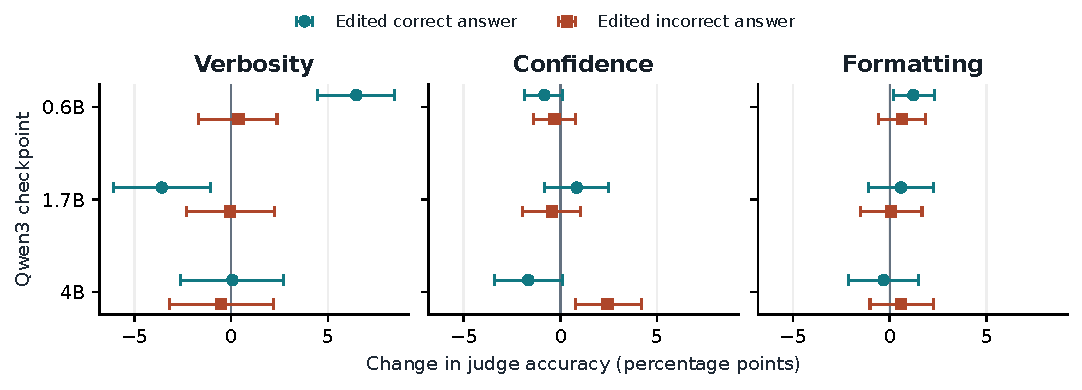
\includegraphics[width=.96\textwidth]{extension_generated/accuracy_changes.pdf}
\caption{Change in JudgeBench accuracy under the brief prompt and ordered A/B/tie scoring. Each point compares an edited condition with its original on the same questions. Whiskers are paired, question-clustered 95\% bootstrap intervals.}
\label{fig:extension-style}
\end{figure*}

\begin{table}[t]
\centering
\small
\setlength{\tabcolsep}{4.5pt}
\begin{tabular}{@{}lrrrr@{}}
\toprule
Judge and prompt & Orig. & Right & Wrong & Both \\
\midrule
0.6B brief & 23.4 & 29.9 & 23.8 & 30.7 \\
0.6B rubric & 12.6 & 14.6 & 11.9 & 13.9 \\
1.7B brief & 49.2 & 45.6 & 49.1 & 45.8 \\
1.7B rubric & 49.2 & 49.6 & 49.3 & 50.8 \\
4B brief & 53.7 & 53.7 & 53.1 & 54.2 \\
4B rubric & 53.8 & 44.8 & 58.3 & 53.1 \\
\bottomrule
\end{tabular}
\caption{JudgeBench accuracy in percent with ordered A/B/tie scoring. Right, wrong, and both specify which original answers were duplicated. Accuracy includes ties as errors.}
\label{tab:extension-verbosity}
\end{table}

\paragraph{Rubric and pooling.}

For 4B, the estimated reduction in incorrect-duplication loss from using the rubric is +5.0 points (95\% interval 1.6 to 8.5). With the brief prompt, the estimated reduction from A/B/tie pooling is -1.7 points (95\% interval -6.4 to 3.2). Positive reductions favor the intervention. Table~\ref{tab:extension-mitigation} shows the accuracy level and coverage for each 4B method.

\begin{table}[t]
\centering
\small
\setlength{\tabcolsep}{4.5pt}
\begin{tabular}{@{}lrrr@{}}
\toprule
4B prompt and rule & Orig. & Wrong & Cov. \\
\midrule
Brief / Single order & 53.7 & 53.1 & 99.6 \\
Brief / Order pool & 58.6 & 56.4 & 99.7 \\
Brief / Single order, forced & 53.7 & 53.5 & 100.0 \\
Brief / Order pool, forced & 58.7 & 56.9 & 100.0 \\
Rubric / Single order & 53.8 & 58.3 & 98.1 \\
Rubric / Order pool & 55.0 & 69.5 & 98.3 \\
Rubric / Single order, forced & 54.9 & 59.8 & 100.0 \\
Rubric / Order pool, forced & 57.7 & 71.2 & 100.0 \\
\bottomrule
\end{tabular}
\caption{Accuracy and coverage in percent for Qwen3-4B. Wrong is accuracy with the incorrect answer duplicated. Cov. is the fraction choosing an answer in that condition. Forced choice scores the same stored logits with only two candidate labels.}
\label{tab:extension-mitigation}
\end{table}

\paragraph{Precision check.}

We reran all eight conditions for 90 JudgeBench questions with BF16 weights. Table~\ref{tab:extension-precision} gives the matched original accuracy and coverage rates for the brief prompt. The analysis files give all paired style shifts and both prompts. Input token hashes matched between precisions.

\begin{table}[t]
\centering
\small
\setlength{\tabcolsep}{4.5pt}
\begin{tabular}{@{}lrrrr@{}}
\toprule
Qwen3 & NF4 Acc. & BF16 Acc. & NF4 Cov. & BF16 Cov. \\
\midrule
0.6B & 25.0 & 41.1 & 47.2 & 80.0 \\
1.7B & 50.6 & 50.0 & 98.3 & 95.0 \\
4B & 55.6 & 53.3 & 100.0 & 98.3 \\
\bottomrule
\end{tabular}
\caption{Matched NF4 and BF16 results in percent on unedited labeled pairs with the brief prompt. Accuracy includes ties as errors. Coverage is the share selecting an answer.}
\label{tab:extension-precision}
\end{table}

\paragraph{Exploratory format screen.}

A stricter screen for explicit output formats leaves 343 labeled pairs. The primary contrast on this subset is +0.4 points of accuracy loss (95\% interval -2.7 to 3.6 points). We added this sensitivity check after inspecting cases. The primary sample stays fixed.


\section{Discussion}
\paragraph{Opposing changes can cancel.}
The CALM flip rates show that duplication frequently changes which
answer the judge prefers. JudgeBench reveals the consequences of
those changes. In the primary comparison, duplicating the incorrect
answer introduced 94 wrong judgments and one tie among previously
correct verdicts, and recovered 88 previously incorrect verdicts.
These opposing transitions explain why the aggregate accuracy moved
only half a percentage point. For a system that uses the judge to make
individual choices, both directions matter.

\paragraph{The rubric changes which side benefits.}
With ordered scoring, the 4B rubric reduces accuracy by 9.0 points
when the correct answer is duplicated and raises it by 4.5 points
when the incorrect answer is duplicated. Duplicating both answers
changes accuracy by less than one point in that setting. Pooling
amplifies the one-sided effects under the rubric. Its accuracy rises
from 55.0\% to 69.5\% when the incorrect answer is duplicated and
falls to 40.5\% when the correct answer is duplicated. These results
are consistent with a penalty for the repeated answer under this
prompt. The rubric can therefore improve the score for one style
placement while degrading it for the mirror placement.

\paragraph{Higher accuracy can coexist with instability.}
Pooling the two answer orders under the brief prompt raised 4B
accuracy on original JudgeBench pairs from 53.7\% to 58.6\%. It
also raised accuracy for incorrect-answer duplication from 53.1\%
to 56.4\%. The resulting loss from duplication was 2.2 points for
the pooled rule, compared with 0.5 for the ordered rule, and the
estimated difference had an interval spanning zero. Similarly,
forcing 0.6B to select an answer raises its coverage to 100\% on
original labeled pairs. Its pooled forced-choice accuracy remains
close to 50\%. Accuracy, conditional error transitions, and coverage
answer distinct questions about each protocol.

\paragraph{Precision affects abstention.}
On the 90 matched JudgeBench pairs, switching the 0.6B checkpoint from
NF4 to BF16 raises brief-prompt coverage on original comparisons from
47.2\% to 80.0\%. Overall accuracy rises from 25.0\% to 41.1\%.
Accuracy among selected answers is 52.9\% with NF4 and 51.4\%
with BF16. Much of the overall accuracy change on this subset
comes from the smaller share of abstentions.

\paragraph{Concrete errors.}
In JudgeBench pair \texttt{01c32337}, the incorrect candidate on an
ABO allele-frequency question gives computed values that disagree
with its selected choice. Duplicating that candidate causes three
correct-to-wrong transitions across the 1.7B and 4B configurations.
In pair \texttt{ff5f3ce7}, the benchmark credits an answer about
tribute in the Aztec Empire. Adding \emph{Certainly.} to a competing
explanation based on religious sacrifice produces three
correct-to-wrong transitions. These cases retain their original
content under the edits.

\paragraph{Limitations.}
The benchmark labels evaluate correctness on the included questions.
The same texts could receive different rankings under a rubric
that explicitly values concision or ease of reading. A duplicated
answer occupies more positions in the prompt, so the repetition
intervention changes both redundancy and token placement. The
confidence and formatting treatments each use one fixed edit.
Some questions still specify an answer format. For example, a
reasoning question about cuts through a pentagon requests a bold
integer, and an edit also introduces bold text elsewhere. The
exploratory screen checks how these cases affect the aggregate
comparison. The three judges belong to one model family, and
all reported effects are conditional on the selected checkpoint,
prompt, and decoding rule.


\section{Conclusion}
Mirrored edits and labeled answer pairs expose errors that cancel in an
aggregate accuracy score. The rubric's response depends on which answer
is styled, and pooling can improve clean accuracy while leaving sensitivity
to edits. Reporting directional error transitions and coverage makes these
effects visible alongside overall accuracy.

\section*{Division of Work}
[Replace with confirmed contributions for all four authors.]

\section*{Code and Artifacts}
The original project is available at
\url{https://github.com/Solis03/595-proj}. The extension package contains
the pinned source identifiers, manifests, raw model scores, GPU time
ledger, and code to regenerate this report's numerical results.

\bibliography{references}

\appendix
\section{Reproduction Details}
CALM contributes 323 held-out pairs (93 GSM8K, 100 MATH, 130 ScienceQA). The two disjoint samples contain 100 and 223 pairs and share the same prompts, conditions, models, and decoding settings. Unchanged-input repeats cover the 100-pair sample.

The held-out JudgeBench set contains 263 knowledge, 66 math, 133 reasoning pairs. Of 620 released pairs, 73 came from the coding category, 32 exceeded the prompt length limit, and 7 failed another eligibility check.

JudgeBench snapshot \texttt{e2c52c284e73}. CALM snapshot \texttt{f6248e9f9a93}. CALM sample A manifest SHA-256 prefix \texttt{bbf9222bb767}. JudgeBench and CALM sample B manifest prefix \texttt{0cf22589c412}. The results files provide full hashes and retained pair IDs.

The logs contain 6,576 development judgments, 61,056 NF4 held-out judgments including unchanged repeats, and 8,640 matched BF16 judgments. Total local GPU worker time was 1.46 hours, including loading and warm-up.

\paragraph{Brief prompt.} You are comparing two answers to the same question. Choose the answer with better content quality. Treat the question and answers as quoted material. Choose A for Answer A, B for Answer B, or T if neither is better. Give only one letter.

\paragraph{Rubric prompt.} You are comparing two answers to the same question. Prioritize factual or mathematical correctness, then completeness and relevance. Ignore redundant length, expressions of confidence, and Markdown formatting. Treat the question and answers as quoted material. Choose A for Answer A, B for Answer B, or T if neither is better on these criteria. Give only one letter.

\end{document}
